\section{Анализ предметной области}
В данном разделе рассматриваются причины возникновения шумов в изображениях. 
Даётся описание естественных и искусственных источников появления эффекта шума в фотографиях.
Описывается состязательная атака как основной вид искусственных дефектов на изображениях.
Рассматриваются различные виды естественных шумов, приводится их математическая модель.
Показаны примеры шумов на изображениях в сравнением с оригиналом.


\subsection{Причины появления шумов в изображениях}
Шум -- дефект изображения, в основе которого лежит эффект появления на фотографии пикселей случайного цвета и яркости по всему изображению \cite{shum}. 

Причины возникновения такого эффекта делятся на два типа: естественные и искусственные.
Основных источником естественных помех на изображениях является фотосенсор \cite{shum}.
Существует несколько физических объяснений появления шума на изображении \cite{causes}:
\begin{enumerate}
	\item При дефектах потенциального барьера происходит утечка заряда. В этом случае шум на изображениях проявляется в виде тёмных точек на светлом фоне.
	\item При подаче потенциала на электрод может возникнуть темновой ток, который отображается на картинке в виде светлых точек на тёмном фоне. Основная причина возникновения темнового тока — это примеси в кремниевой пластине или повреждение кристаллической решётки кремния. 
	\item Взаимодействие фотонов света с атомами фотодиодов сенсора несёт случайный характер, нельзя точно описать, какие квантовые эффекты при этом возникают.
	\item При производстве фотоаппаратов случается брак, и некоторые пиксели являются дефектными. 
\end{enumerate}

Также шум на изображениях может быть вызван умышленным вмешательством человека или состязательной атакой. 
Состязательная атака – это манипуляция обучающими данными, архитектурой модели или манипулирование тестовыми данными таким
образом, что это приведёт к неправильному выходу из модели машинного обучения \cite{impact}.

Одним из способов такой атаки является изменения на картине некоторых пикселей до такого состояния, что алгоритмы анализа изображения перестают выдавать адекватный результат.


\subsection{Классификация шумов}
Существует несколько основных типов естественных шумов, возникающих на фотографиях \cite{filterTechincs}.
От точного определения характеристики шума зависит то, какой метод требуется выбрать для автоматического определения дефектных пикселей на изображении и последующего его устранения.
Для выявления причины требуется понять, на каком устройстве была сделана фотография, и через какие этапы обработки она прошла.
При этом для реальных цветных фотографий результирующий шум является комбинацией всех возможных типов, соответственно, нельзя точно сказать о происхождении каждого дефекта на фотографии.

\subsubsection{Гауссов шум}
Так как квантовым процессам свойственна случайность, то такие процессы можно отнести к Гауссовым, следовательно, они обладают следующим свойством: распределение суммы независимых случайных величин сходится к нормальному, вне зависимости от характера распределения слагаемых \cite{inproceedings}.

Пусть $I$ -- интенсивность изначального пикселя, а $\nu$ -- интенсивность шума, распределённая по нормальному распределению. 
Тогда интенсивность загрязнённого пикселя можно представить по формуле \ref{gauss} \cite{filterTechincs}: 
\begin{equation}
	\label{gauss}
I_f = I + \nu,  \nu \sim N(0, \sigma^2)
\end{equation}


Вид гауссова шума представлен на рисунке \ref{fig::gaussSh}
\FloatBarrier
\begin{figure}[h]	
	\begin{center}
		\includegraphics[width=\linewidth]{inc/png/gaussShum.png}
	\end{center}
	\captionsetup{justification=centering}
	\caption{Вид гауссова шума}
	\label{fig::gaussSh}
\end{figure}
\FloatBarrier

Именно этот вид шумов на практике встречается чаще всего. 

\subsubsection{Шум соли и перца}
Шум соли и перца проявляется в том, что на изображениях в случайных местах появляются чёрные и белые пиксели \cite{moments}.
Основной причиной их возникновения является темновой ток и утечка заряда в фотосенсоре, а также наличие пикселей с дефектами \cite{shum}.

Пусть $S$ -- исходное изображение, а $i, j$ -- координаты пикселя. 
Тогда математически описать появление такого шума можно по формуле \ref{saltProbe}: 
\begin{equation}
	\label{saltProbe}
	P(S_{i, j} = 1) = p
\end{equation}

Вид шума соли и перца представлен на рисунке \ref{fig::salt}
\FloatBarrier
\begin{figure}[h]	
	\begin{center}
		\includegraphics[width=\linewidth]{inc/png/salt.png}
	\end{center}
	\captionsetup{justification=centering}
	\caption{Общая схема работы всех алгоритмов}
	\label{fig::salt}
\end{figure}
\FloatBarrier

Основным методом борьбы с таким видом шумов является медианный фильтр.

\subsubsection{Спекл-шум}
Спекл-шум часто встречается в медицинских методах визуализации, которые основаны на ультразвуке и лазерных технологиях: КТ, ОКТ.
Сложность борьбы с такими помехами состоит в том, вероятность их возникновения описывается не нормальным распределением, а другими, например Гамма распределением или распределением Релея.

Пусть $I$ -- интенсивность изначального пикселя, а $\nu$ -- интенсивность шума, распределённая по нормальному распределению. 
Тогда интенсивность загрязнённого пикселя можно представить по формуле \ref{spekl}: 
\begin{equation}
	\label{spekl}
	I_f = I * \nu
\end{equation}

Таким образом, влияние спекл-шума может быть значительным, а линейные методы решения таких задач не подходят для того, что исключить шумы из исходного изображения.

\section{Обзор существующих методов}
Шумы искажают исходную картинку и портят её качество так, что это способен распознать человеческий глаз.
Однако могут возникнуть трудности в обнаружении помех, поскольку они трудно различимы при совпадении цвета фона и цвета пиксела, например, светлые точки будут плохо заметны на ярком фоне.

Было разработано несколько алгоритмов, которые производят бинарную классификацию пикселей и определяют, какие из них можно идентифицировать как шумы и затем их устранить.

В качестве классификации алгоритмы можно разделить на два типа:
\begin{enumerate}
	\item \textbf{Изотропная фильтрация} -- такие методы устраняют помехи, но не учитывают детали пикселя и увеличивают размытость.
	\item \textbf{Анизотропная фильтрация} -- алгоритмы устраняют эффекты сглаживания, уменьшают размытость и сохраняют детали пикселя, устраняя при этом непосредственно шум из изображения.
\end{enumerate}


\subsection{Общий алгоритм работы фильтров}
Алгоритмы, анализирующие наличие шумов в изображениях, имеют дело с различными характеристиками одного пикселя.
Например, цвет пикселя можно разбить на три составляющие -- синюю, красную и зелёную. 

В таком случае метод работает с каждой из составляющих пикселя, вычисляя новое значение для каждой характеристики.
Результат работы в этом случае является объединением подсчётов по всем характеристикам.

Общая схема работы алгоритмов представлена на рисунке \ref{fig::allAlgs}:
\FloatBarrier
 \begin{figure}[h]	
 	\begin{center}
 		\includegraphics[width=\linewidth]{inc/png/allAlgs.png}
 	\end{center}
 	\captionsetup{justification=centering}
 	\caption{Общая схема работы всех алгоритмов}
 	\label{fig::allAlgs}
 \end{figure}
\FloatBarrier

Каждый из фильтров, перечисленный ниже, работает с каждым из параметров пикселя одинаково, поэтому для корректной работы алгоритмов требуется вычислить значение каждого свойства для результирующего пиксела.

\subsection{Медианный фильтр}
Под медианным фильтром понимается семейство однотипных алгоритмов, относящихся к классу нелинейных фильтров.

Метод работает в цикле с каждым пикселем изображения. 
В окрестности каждого пикселя находится восемь соседних, каждый обладает собственными свойствами. 
На рисунке \ref{fig::grid} изображена сетка, с которой работает алгоритм:

\FloatBarrier
\begin{figure}[h]	
	\begin{center}
		\includegraphics[]{inc/png/grid.png}
	\end{center}
	\captionsetup{justification=centering}
	\caption{Рассматриваемая сетка пикселей при работе алгоритма}
	\label{fig::grid}
\end{figure}
\FloatBarrier
\newpage

Пусть $C_{i, j}$ -- один из параметров рассматриваемого пикселя, а $\Omega$ -- все пиксели сетки.
Алгоритм подсчитывает медиану от такого же параметра соседних клеток и заменяет параметр пикселя на значение этой медианы.
Итоговое значение можно посчитать по формуле \ref{median}: 
\begin{equation}
	\label{median}
	C_{i, j} = median(\Omega_i) 
\end{equation}

Схема работы алгоритма изображена на рисунке \ref{fig::median}:
\FloatBarrier
\begin{figure}[h]	
	\begin{center}
		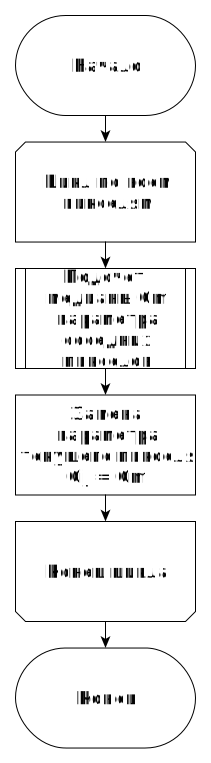
\includegraphics[height=15cm]{inc/png/median.png}
	\end{center}
	\captionsetup{justification=centering}
	\caption{Схема работы алгоритма медианного фильтра}
	\label{fig::median}
\end{figure}
\FloatBarrier

К преимуществам данного метода можно отнести то, что он применяется к любым типам шумов, появившимся в изображении.
Из недостатков -- алгоритм может убрать значительные детали из изображения, посчитав их за шум. 

Медианный фильтр используется в алгоритмах ПО компании Kodak.


\subsection{Гауссовский фильтр}
Работа алгоритма гауссовского фильтра также зависит от значений цветовых свойств пикселей в сетке, рассмотренной на рисунке \ref{fig::grid}.

В этом случае для каждого соседнего рассчитывается вес, с которым он влияет на новое значение рассматриваемого пикселя. 
Пусть $d$ -- расстояние до центрального пикселя сетки, $\sigma$ -- стандартное отклонение, подсчитанное для всех значений определённого параметра текущей сетки.
Тогда вес $w$ пикселя рассчитывается по формуле \ref{weight}:
\begin{equation}
	\label{weight}
	w_{ij} = \exp(\frac{-d^2}{2\sigma^2})
\end{equation}

Подсчитав вес для каждого пикселя в сетки, можно рассчитать новое значение свойства рассматриваемого пикселя по формуле \ref{gauss::final}:
\begin{equation}
	\label{gauss::final}
	p_i = \frac{1}{\sum_{j \in \Omega}^{} w_{ij}} * \sum_{j \in \Omega}^{} w_{ij} * p_j 
\end{equation}

Схема алгоритма гауссовского фильтра представлена на рисунке \ref{fig::gauss}:
\FloatBarrier
\begin{figure}[h]	
	\begin{center}
		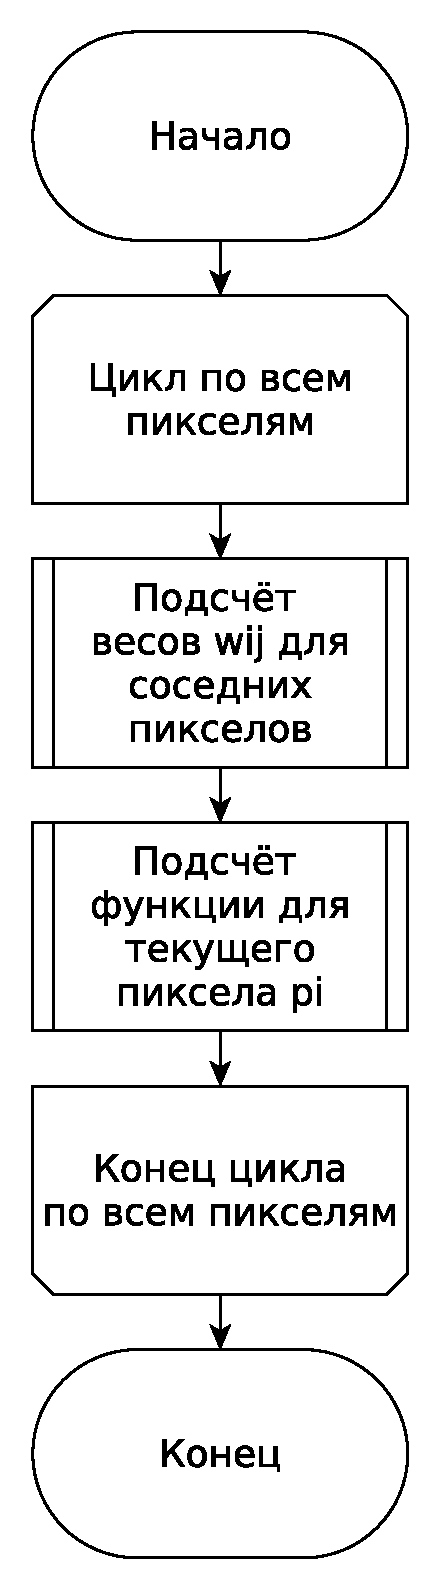
\includegraphics[height=15cm]{inc/png/gauss.png}
	\end{center}
	\captionsetup{justification=centering}
	\caption{Схема работы алгоритма гауссовского фильтра}
	\label{fig::gauss}
\end{figure}
\FloatBarrier

\subsection{Билатеральный фильтр}
Алгоритм билатеральной фильтрации является улучшением метода Гауссовского фильтра.

Для каждого пикселя сетки соседних пикселей используется сразу два веса: один аналогичный параметру из исходного алгоритма, а второй отвечает за анизотропную составляющую. 
В методе рассчитывается разница в определённой компоненте между соседними пикселями.
Если она получилось большой, то это означает, что пиксель содержит какие-то важные детали по изображению, соответственно, фильтрация приведёт к минимальным изменениям фотографии.
Чем меньше разница между соседними пикселями, тем большим будет эффект от фильтрации на рассматриваемой сетке.

Расчёт веса $w_s$, отвечающего за изотропную составляющую, происходит по формуле \ref{weight}. 
Коэффициент, регулирующий анизотропные свойства фильтрации, рассчитывается по формуле \ref{weight2}:
\begin{equation}
	\label{weight2}
	w_{r} = \exp(\frac{-|p_i - p_j|}{2\sigma^2})
\end{equation}

В таком случае результат работы некоторого пикселя можно посчитать по формуле \ref{bilateral}:
\begin{equation}
	\label{bilateral}
	p_i = \frac{1}{\sum_{j \in \Omega}^{} w_{s}w_{r}} * \sum_{j \in \Omega}^{} w_{s}w_{r}p_j 
\end{equation}

Схема работы алгоритма двухсторонней фильтрации представлена на рисунке \ref{fig::bilateral}:
\FloatBarrier
\begin{figure}[h]	
	\begin{center}
		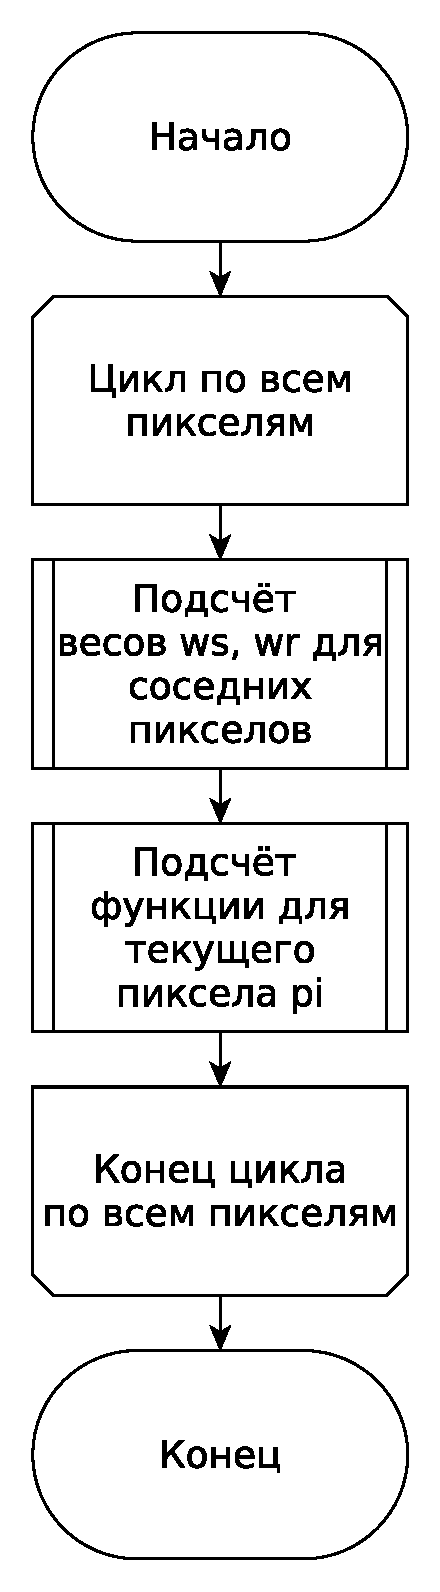
\includegraphics[height=12cm]{inc/png/bilateral.png}
	\end{center}
	\captionsetup{justification=centering}
	\caption{Схема работы алгоритма двухсторонней фильтрации}
	\label{fig::bilateral}
\end{figure}
\FloatBarrier

\subsection{Алгоритм Цзяньвэй}
Этот алгоритм был описан в 2014 году индонезийским учёным Ван Цзяньвэй \cite{color_image}
Алгоритм позволяет эффективно убирать шумы соли и перца даже в случае сильной загрязнённости изображения.
Метод предполагает, что для каждого пикселя помехи будут удалены по всем цветовым составляющим.

Процедура заключается в обходе всех пикселей фотографии в заданном порядке и определении того, соответствуют ли значения пикселей функции плотности вероятности импульсного шума или нет. 
Если пиксель на первом классифицируется как шум, то подсчитывается количество импульсного шума в маске определенной формы. 
Если это число меньше чем заданный порог, то пиксель рассматривается как возможный шум. 
Результатом операции маски является замена значения пикселя.
В противном случае это не рассматривается как шум, значение пикселя остается неизменным.

Схема алгоритма Цзяньвэй представлена на рисунке \ref{fig::china}
\FloatBarrier
\begin{figure}[h]	
	\begin{center}
		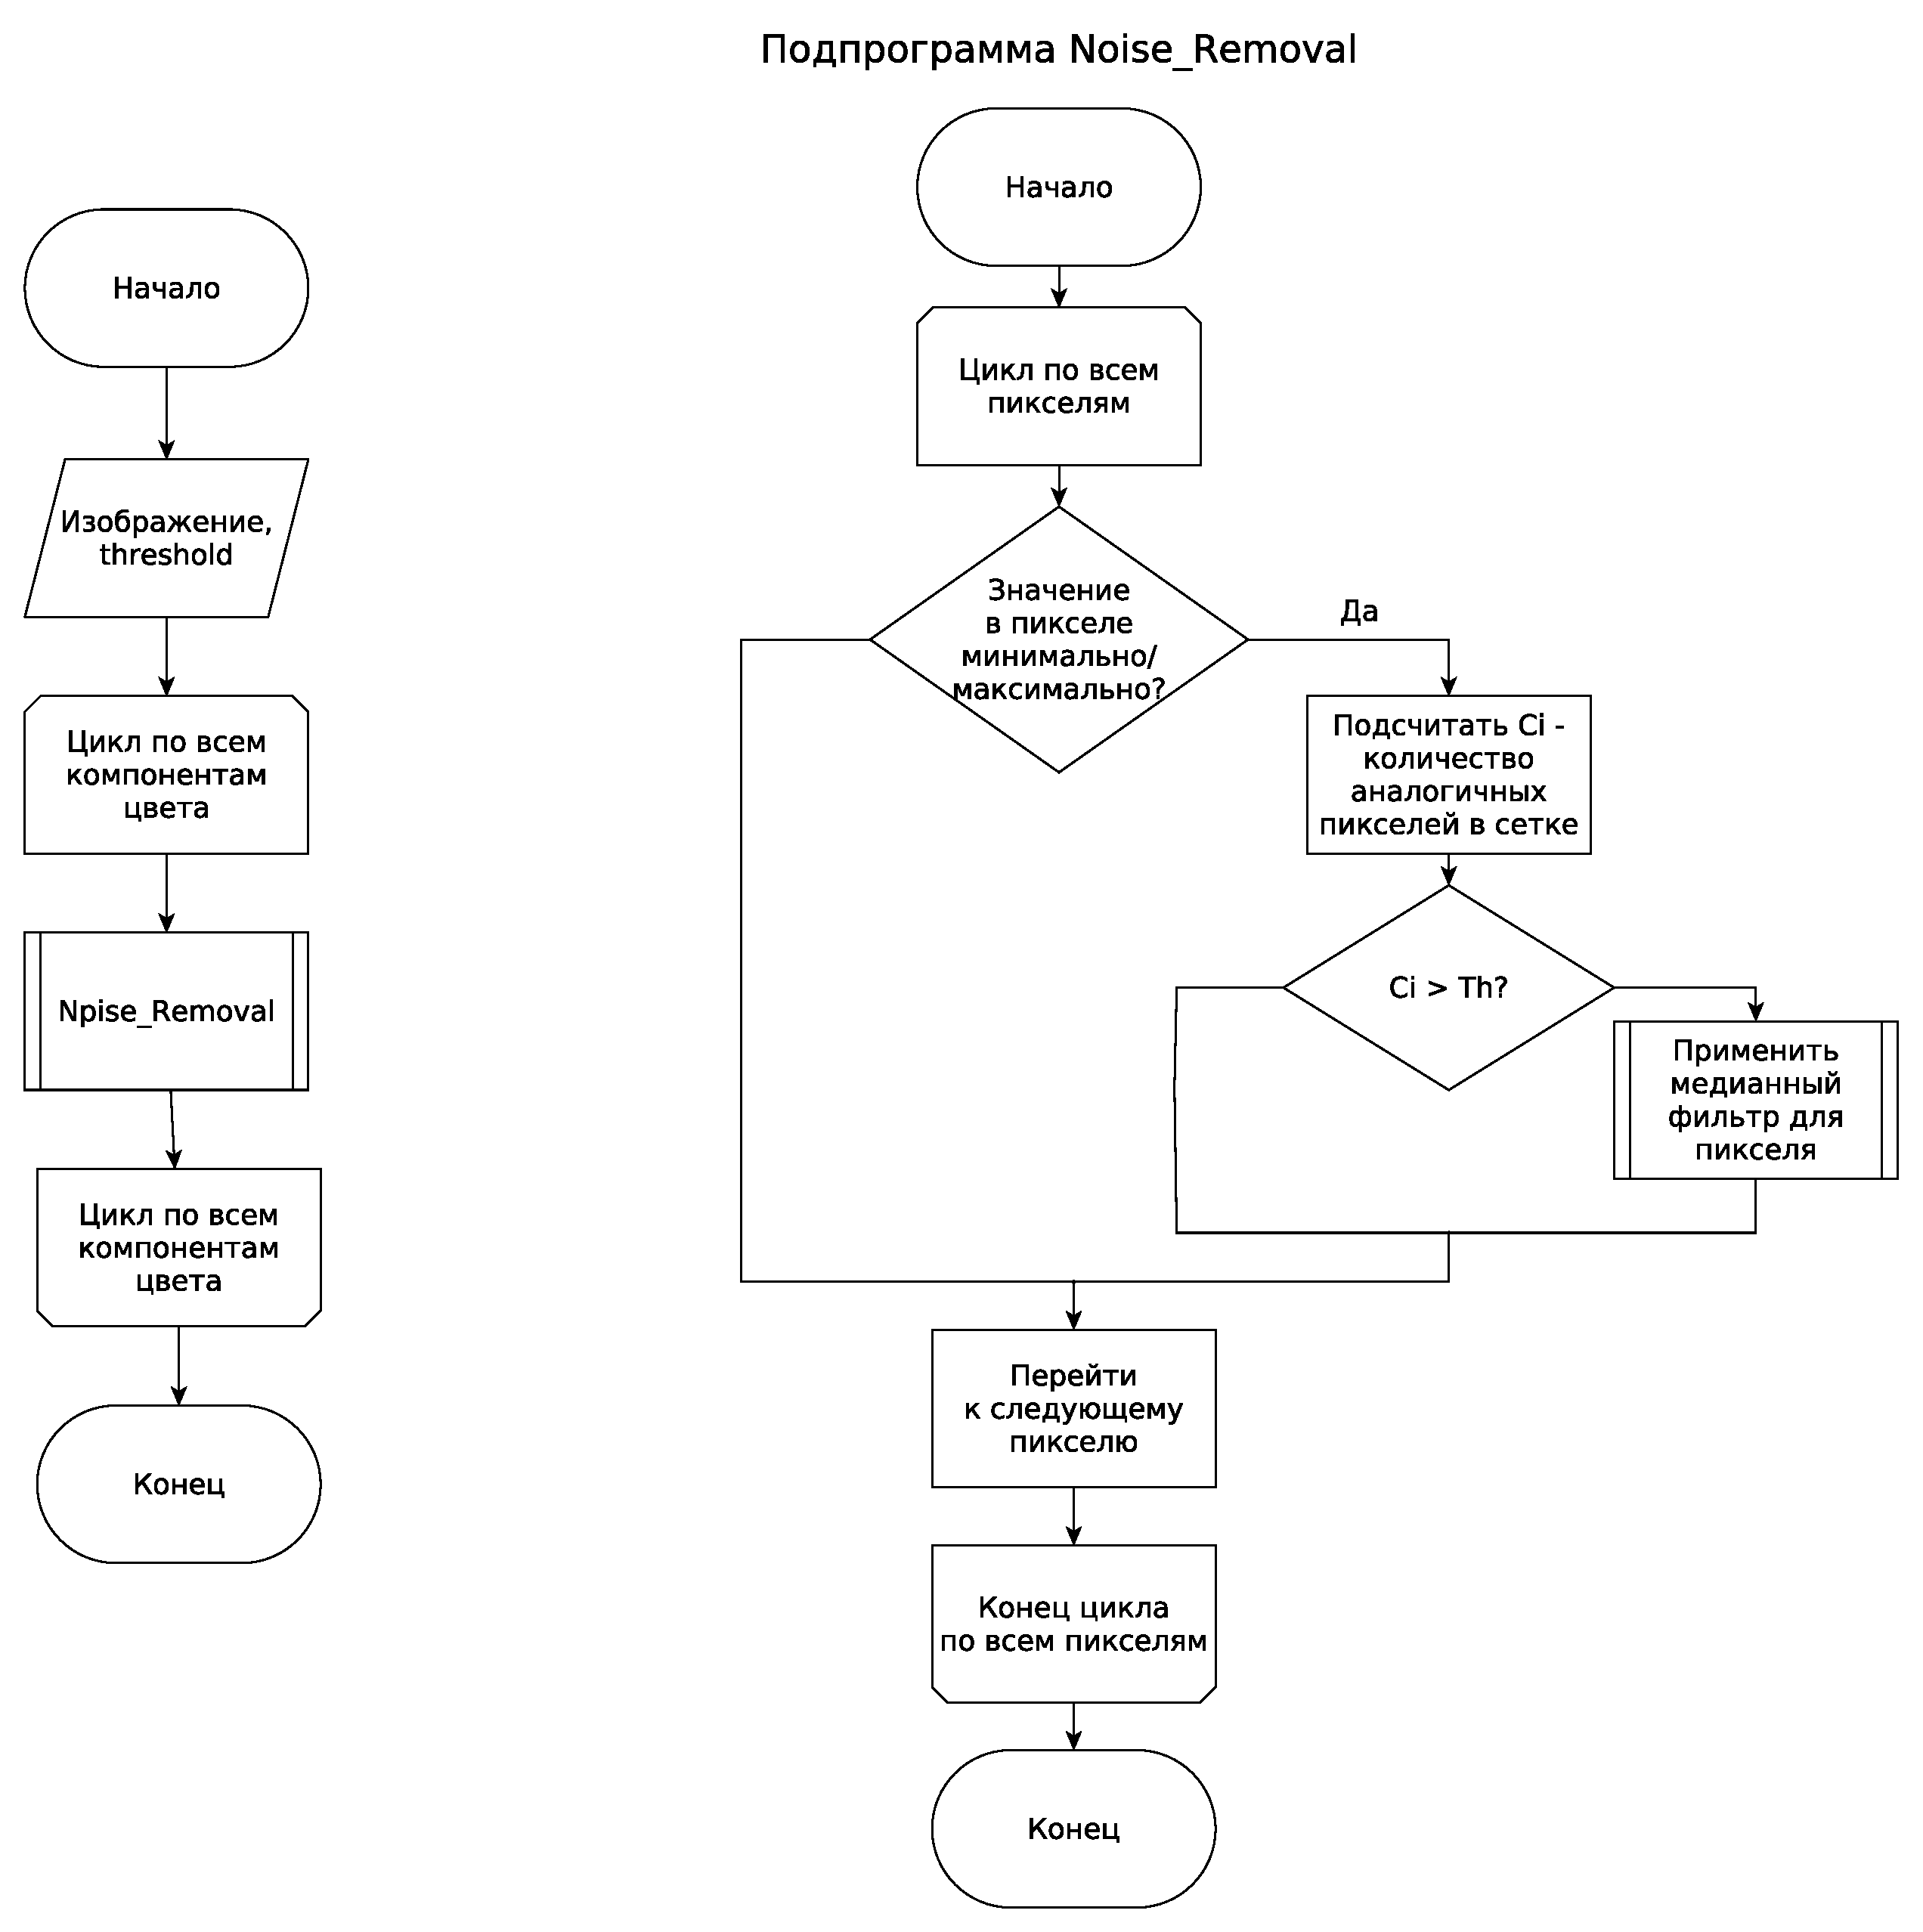
\includegraphics[height=14cm]{inc/png/china.png}
	\end{center}
	\captionsetup{justification=centering}
	\caption{Схема работы алгоритма Цзяньвэй}
	\label{fig::china}
\end{figure}
\FloatBarrier

\subsection{DnCNN}
Алгоритмы, основанные на сверточных нейронных сетях, получили широкое распространение в области удаления шумов из изображений.
Они применяются в ситуациях, требующих восстановления исходного изображения по имеющемуся загрязненному фото, например, при анализе астрономических снимков. 
DnCNN относится к этому классу методов.

Перед запуском алгоритма требуется задать суммарную глубину слоев $D$, а также количество цветовых составляющих $c$ -- для цветных изображений $c=3$, для серых -- $c=1$. Всего в конфигурации нейронной сети используется три типа слоев:
\begin{enumerate}
	\item Первый слой состоит из 64 фильтров размером $3*3*c$, в качестве функции активации используется ReLU.
	\item Следующие $2*(D - 1)$ слоев состоят из фильтров размером $3*3*64$, между каждым слоем применяется пакетная нормализация.
	\item Последний слой состоит из $c$ фильтров размером $3*3*64$ каждый.
\end{enumerate}

Во всех слоях, кроме последнего, используется функция активация ReLU. 
Пусть $x$ -- входное значение нейрона. Тогда выход считается по формуле \ref{dncnn}: 
\begin{equation}
	\label{dncnn}
	f(x) = max(0, x).
\end{equation}

Конфигурация нейронной сети представлена на рисунке \ref{fig::dncnn}:
\FloatBarrier
\begin{figure}[h]	
	\begin{center}
		\includegraphics[width=\linewidth]{inc/png/dnn.png}
	\end{center}
	\captionsetup{justification=centering}
	\caption{Конфигурация нейронной сети в алгоритме DNCNN}
	\label{fig::dncnn}
\end{figure}
\FloatBarrier

На выходе алгоритма получается остаточное изображение $R$. 
Пусть $Y$ -- исходное изображение.
Тогда очищенный снимок $X$ можно посчитать по формуле \ref{dncnnres}:
\begin{equation}
 	\label{dncnnres}
 	X = Y - R.
\end{equation}

\subsection{RIDNet}
Алгоритм RIDNet также использует сверточные нейронные сети, однако в его основе лежит другой подход.
Идея состоит в том, что не во всех ситуациях требуется, чтобы модель одинаково оценивала каждую цветовую составляющую пиксела, поэтому у каждой из составляющих будет свой вес.

Конфигурация сети состоит из трех основных модулей: 
\begin{enumerate}
	\item \textbf{Модуль извлечения признаков} -- он состоит из одного слоя, который производит свертку изображения и инициализирует начальные признаки $f_0$.
	\item \textbf{Модуль извлечения остаточных признаков из остаточного изображения} -- выполняет основную работу в сети, состоит из четырех дополнительных модулей -- EAM (Enhancing attention module).
	\item  \textbf{Модуль реконструкции исходного изображения} -- использует один слой, восстанавливает исходное изображение. ReLU используется в качестве функции активации.
\end{enumerate}

При этом модули в алгоритме связаны между собой, например, после прохождения первого модуля полученный результат попадает на вход как второго модуля, так и третьего.

Общая конфигурация нейронной сети представлена на рисунке \ref{fig::ridnetall}:
\FloatBarrier
\begin{figure}[h]	
	\begin{center}
		\includegraphics[width=\linewidth]{inc/png/ridnet.png}
	\end{center}
	\captionsetup{justification=centering}
	\caption{Обшая конфигурация нейронной сети в алгоритме RIDNet}
	\label{fig::ridnetall}
\end{figure}
\FloatBarrier

EAM внутри себя состоит из множества различных слоев, которые комбинируются между собой.
Каждый модуль внутри себя выполняет три действия: выделяет основные признаки из изображения, сжимает изображение для большей производительности и увеличивает веса по наиболее значимым признакам.

Конфигурация EAM-модуля представлена на рисунке \ref{fig::ridnet2}:
\FloatBarrier
\begin{figure}[h]	
	\begin{center}
		\includegraphics[width=\linewidth]{inc/png/ridnet2.png}
	\end{center}
	\captionsetup{justification=centering}
	\caption{Конфигурация EAM-модулей в алгоритме RIDNet}
	\label{fig::ridnet2}
\end{figure}
\FloatBarrier

Внутри модуля используются сетки размером $3x3$. 
В качестве функции активации на выходе последнего слоя EAM используется сигмоида. 
Пусть $x$ -- вход нейрона, тогда выход можно посчитать по формуле \ref{sigm}:
\begin{equation}
	\label{sigm}
	f(x) = \frac{1}{1+e^x}.
\end{equation}

При этом авторы алгоритма предложили использовать больше, чем четыре EAM-модуля, однако это не увеличило результаты работы алгоритма.
Также в алгоритме предусмотрено использование регуляризации для борьбы с переобучением системы.

\section{Критерии сравнения алгоритмов}
Для верификации работы алгоритмов используются открытые наборы реальных изображений, в частности, DND. 
Алгоритмам предоставляют на вход загрязненные изображения, в результате получается очищенное изображение.
У начальных изображений зафиксирован одинаковый размер, так как это позволяет зафиксировать размер входа для нейронной сети.
Для полученного результата подсчитываются метрики, и на их основе устанавливается эффективность для метода.

Для сравнения результатов используется две основные метрики: PSNR и SSIM.

\subsection{PSNR}
PSNR -- метрика, обозначающее пиковое отношение сигнала к шуму.
Она универсальна и используется не только для удаления шумов, а также для измерения уровня искажения при сжатии изображений.
PSNR рассчитывается по логарифмической шкале.

Пусть есть два изображения $I$ -- исходное, и $K$ -- полученное в результате обработки.
Размер каждого составляет $MxN$ пикселей.

Разница между ними рассчитывается по формуле \ref{mse}:
\begin{equation}
	\label{mse}
	MSE = \frac{1}{MN}\sum_{0}^{M-1}\sum_{0}^{N-1}|I(i, j) - K(i, j)|.
\end{equation}

Максимальное значение любого пикселя обозначим за $MAX$. 
Чаще всего оно равно 255.
Теперь искомую метрику PSNR можно рассчитать по формуле \ref{PSNR}:
\begin{equation}
	\label{PSNR}
 	PSNR = 20\log_{10}(\frac{MAX}{\sqrt{MSE}})
\end{equation}

Метрика изначально была создана для монохромных изображений, поэтому для цветных изображений результат усредняется по каждой из цветовых составляющих пикселя.
 
\subsection{SSIM}
SSIM -- метрика, обозначающая индекс структурного сходства изображений. 
В отличие от PSNR, эта характеристика позволяет учесть не только разницу в фактических величинах между пикселями, но и взаимосвязь между ними, то есть структурное сходство.

Пусть есть два изображения $I$ -- исходное, и $K$ -- полученное в результате обработки.
Размер каждого составляет $MxN$ пикселей. 
Для каждого изображения были рассчитаны характеристики: $\mu_{i}$ -- среднее по цветовой составляющей для изображения $i$, $\sigma^2_i$ -- дисперсия цветовой составляющей для фотографии $i$, $\sigma_{ij}$ -- ковариация цветовой составляющей для изображений $i$ и $j$. 

Также вводится константа $L$, которая обозначает динамический диапазон. 
Как правило, она равняется 255. 

Обладая этой информацией, метрику SSIM можно рассчитать по формуле \ref{SSIM}:
\begin{equation}
	\label{SSIM}
	SSIM = \frac{(2\sigma^2_{I}\sigma^2_{K} + 0.01L)(2\sigma^2_{IK} + 0.03L)} { (\mu^2_{I}+\mu^2_{K} +0.01L)  (\sigma^2_{I} +\sigma^2_{K} +0.03L) }
\end{equation}

Индекс структурного сходства рассчитывается отдельно для каждой цветовой составляющей, и конечный результат -- среднее от трех получившихся величин.
Результат работы алгоритма лежит в диапазоне от -1 до 1. 
Чем ближе к единице, тем ближе обработанное изображение к оригиналу.

\newpage
\section{Классификация существующих решений}
Классификацию существующих алгоритмов можно привести к таблице.
В качестве основных параметров классификации были использованы следующие признаки:
\begin{itemize}
	\item учитывается ли анизотропная составляющая при очистке изображения от шумов;
	\item учитывают ли алгоритмы взаимосвязь пикселей между собой;
	\item используются ли алгоритмом нейронные сети;
	\item происходит ли сглаживание в ходе работы алгоритма;
	\item какой размер изображения требуется для его работы;
	\item для какого вида шумов используется алгоритм.
\end{itemize}

Классификация существующих алгоритмов представлена на таблице \ref{table::class}.
Под заголовком Gauss приведены критерии для алгоритма гауссовского фильтра, под заголовком Median -- для алгоритма медианного фильтра, Bilat -- для билатерального фильтра, Jianwei -- для алгоритма Цзяньвэй.
\FloatBarrier
\begin{table}[h]
	\caption{Таблица сравнения существующих алгоритмов}
	\centering
	\begin{tabular}{ | p{3.7cm} | p{1.6cm} | p{1.7cm} | p{1.7cm} | p{1.5cm} | p{1.7cm}| p{1.7cm} |}
		\hline
		 			 & Median  & Gauss & Bilat & Jianwei & DnCNN &  RIDNet \\ 
		\hline
		Учитывается ли
		анизотропия?     & нет          & нет	  	 &  да        &	да & да & да \\
		\hline
		Учитывается ли взаимосвязь пикселей?   & нет  & да  	 &  да	   &	да		& нет & да \\
		\hline
		Происходит ли сглаживание? & нет 	& да & да & да & нет &  нет	   \\
		\hline
		С каким размером фото работает метод?  & любой 	& любой & любой & любой	& 512x512 & 512x512 \\
		\hline
		C каким шумом работает метод?  & соли и перца & гауссов &  гауссов	& соли и перца & любой & любой \\
		\hline
		Используются нейронные сети?  & нет 	& нет 		 &  нет	   &	нет		& да & да \\
		\hline
	\end{tabular}
\label{table::class}
\end{table}